\let\negmedspace\undefined
\let\negthickspace\undefined
\documentclass[journal]{IEEEtran}
\usepackage[a5paper, margin=10mm, onecolumn]{geometry}
%\usepackage{lmodern} % Ensure lmodern is loaded for pdflatex
\usepackage{tfrupee} % Include tfrupee package

\setlength{\headheight}{1cm} % Set the height of the header box
\setlength{\headsep}{0mm}  % Set the distance between the header box and the top of the text

\usepackage{gvv-book}
\usepackage{gvv}
\usepackage{cite}
\usepackage{amsmath,amssymb,amsfonts,amsthm}
\usepackage{algorithmic}
\usepackage{graphicx}
\usepackage{textcomp}
\usepackage{xcolor}
\usepackage{txfonts}
\usepackage{listings}
\usepackage{enumitem}
\usepackage{mathtools}
\usepackage{gensymb}
\usepackage{comment}
\usepackage[breaklinks=true]{hyperref}
\usepackage{tkz-euclide} 
\usepackage{listings}
% \usepackage{gvv}                                        
\def\inputGnumericTable{}                                 
\usepackage[latin1]{inputenc}                                
\usepackage{color}                                            
\usepackage{array}                                            
\usepackage{longtable}                                       
\usepackage{calc}                                             
\usepackage{multirow}                                         
\usepackage{hhline}                                           
\usepackage{ifthen}                                           
\usepackage{lscape}
\begin{document}

\bibliographystyle{IEEEtran}
\vspace{3cm}

\title{9.2.3}
\author{EE24BTECH11014 - Deepak Ahirwar}

% \maketitle
% \newpage
% \bigskip
{\let\newpage\relax\maketitle}

\renewcommand{\thefigure}{\theenumi}
\renewcommand{\thetable}{\theenumi}
\setlength{\intextsep}{10pt} % Space between text and floats

\textbf{Question:}\\
For the Differential Equation $\frac{dy}{dx}+ \sin{x}=0$, verify that $y = \cos{x}+C$ is a solution of the differential equation.

\solution:
We are given the first-order ordinary differential equation:
\begin{align}
\frac{dy}{dx} + \sin x &= 0
\end{align}

This is a separable differential equation. We can rewrite it as:
\begin{align}
\frac{dy}{dx} &= -\sin x
\end{align}

Now, we integrate both sides with respect to $x$:
\begin{align}
\int \frac{dy}{dx} \, dx &= \int -\sin x \, dx \\
\int dy &= -\int \sin x \, dx
\end{align}
\begin{align}
 \implies y &= \cos x + C
\end{align}

where $C$ is the constant of integration.

Therefore, the general solution to the given differential equation is:
\begin{align}
y(x) = \cos x + C
\end{align}

\textbf{Computational Solution:}\\
Using classical defination of derivative we get,\\
\begin{align}
    f\prime\brak{x} &= \frac{f\brak{x+h}-f\brak{x}}{h}\\
    \implies f\brak{x+h} &= f\brak{x} + f\prime\brak{x}h
\end{align}
For  $y = f\brak{x}$, we can get the  points of the required graph by iterating the equation obtained in (8) where values of $x$ increases in each iteration by $h$ and obtaining the y-coordinate of it.\\
For,
\begin{align}
x_0 &= 0\\
y_0 &= 1\\
h &= 0.001
\end{align}
Using Euler Method, we get difference equation,
\begin{align}
y_{n+1} &= y_n + h\frac{dy}{dx}\Big|_{\brak{x_n,y_n}}\\
	y_{n+1} &= y_n - h\sin {x_n}\\
x_{n+1} &= x_n + h
\end{align}

\begin{figure}[h]  % The 'h' means 'here' (positioning)
    \centering  % Centers the figure
    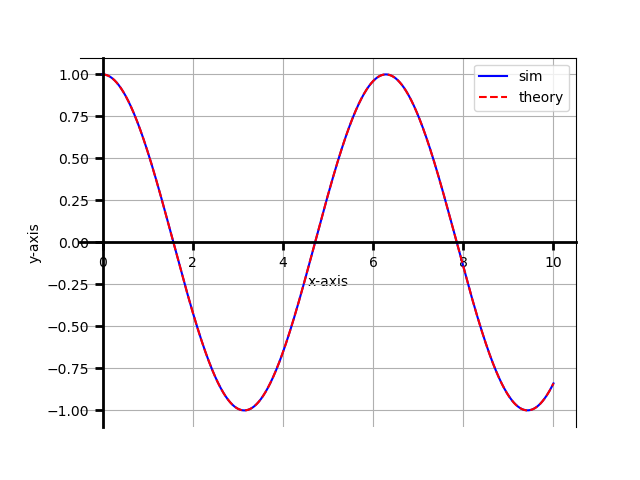
\includegraphics[width=\columnwidth]{fig/Figure_1.png}  
    \caption{Verification}
    \label{fig:example}  % Label for referencing
\end{figure}
 




\end{document}
